\section{Expérience C2} \label{expC2}
  \subsection{Objectif}
    Comprendre de quelles manières un réseau de neurone connexionniste peut parier sur ses propres résultats
    à partir de ses représentations personnelles.

    
    Réalisation de la seconde expérience de l'article \cite{Cleeremans_2007} sur des données réelles.
  
  
  \subsection{Architecture}
    \paragraph{Description}
      Un premier réseau de perceptron multicouche apprend à discrétiser des chiffres représentés
      par 256 (16x16) neurones d'entrées. Il est composé d'une couche cachée de 20 ou 100 neurones.
      
      Un second réseau de perceptron multicouche apprend à parier sur la qualité de la réponse
      du premier réseau à partir de sa couche cachée.
      
      L'apprentissage du second réseau, n'affecte pas les poids entre la couche d'entrée et la 
      couche cachée du premier réseau.

    \paragraph{Schéma}
      \begin{center}
	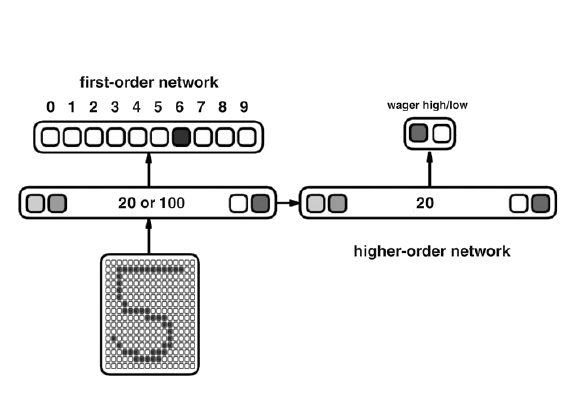
\includegraphics[width=240px]{data/expC2/schema.png}
      \end{center}
      
    \paragraph{Paramètres}
      \begin{center}
	\begin{tabular}{lr}
	  \begin{minipage}{230px}
	    \begin{itemize}
	      \item momentum : 0.5 sur le premier réseau
	      \item momentum : 0. sur le second réseau
	      \item taux d'apprentissage : 0.15 sur les 2 réseaux
	      \item \textbf{1600 formes} de chiffres différents présentées (shuffle) \cite{Handwritten_256}
	      \item apprentissage 50 (formes) x 300 (époques)
	      \item utilisation de biais
	      
	    \end{itemize}
	  \end{minipage}
	  &
	  \begin{minipage}{230px}
	    \begin{itemize}
	      \item poids initialisés sur [-1 ; 1] pour le premier réseau
	      \item poids initialisés sur [-0.25 ; 0.25] pour le second réseau
	      \item taux d'apprentissage constant
	      \item entrées valent 0 ou 1
	      \item sigmoïde à température 1
	    \end{itemize}
	  \end{minipage}
	\end{tabular}
      \end{center}


  
  \newpage
  \subsection{Résultats}
    \paragraph{Principaux}
      Analyse des performances
      \begin{center}
	\begin{tabular}{lr}
	  \hspace*{-1cm}
	  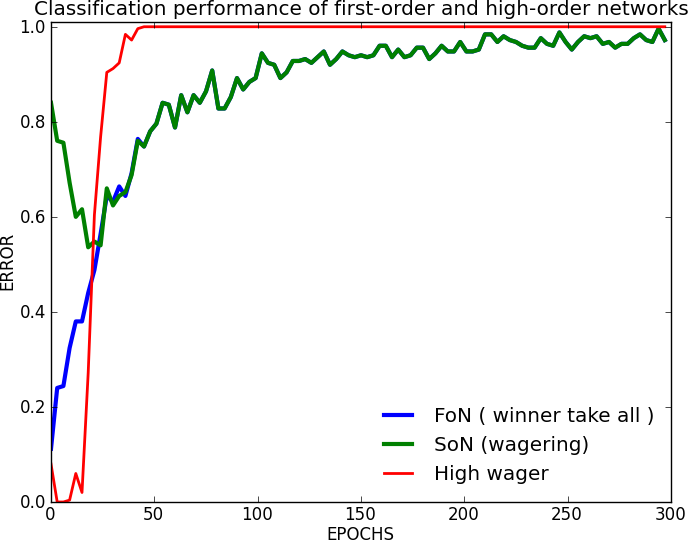
\includegraphics[width=250px]{data/expC2/perf_20.png}
	  &
	  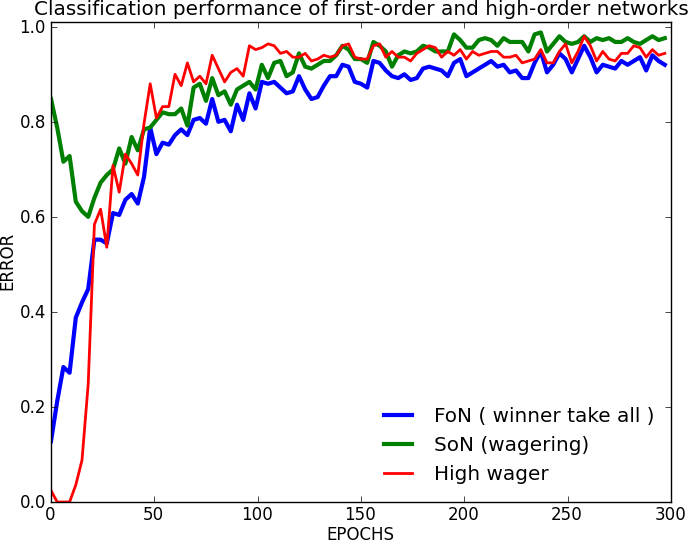
\includegraphics[width=250px]{data/expC2/perf_100.png} \\
	  
	  20 neurones en couche cachée
	  &
	  \hspace*{-1cm}
	  100 neurones en couche cachée
	\end{tabular}
      \end{center}
      \subparagraph{Notes}
	\begin{itemize}
	  \item la courbe rouge représentent le taux de paris hauts du second réseau
	\end{itemize}
      \subparagraph{Conclusion}
	\begin{itemize}
	  \item dans les 2 cas, le premier réseau réussit à apprendre sa tâche de classification
	  \item lorsque le nombre de neurones dans la couche cachée est faible, l'apprentissage de la tâche est optimal, il ne peut plus être amélioré
	  
	  Ainsi le second réseau se contente de parier haut.
	  \item lorsque le nombre de neurones dans la couche cachée est élevé, l'apprentissage peut être amélioré, le second réseau 
	  le remarque et peut accorder son taux de paris hauts avec le taux de succès du premier réseau.
	  
	  Remarquons tout de même qu'avec l'amélioration du second réseau, on ne peut pas dépasser un réseau optimal, seulement l'égaler
	\end{itemize}
    \paragraph{Secondaires}
      RMS
      \begin{center}
	\begin{tabular}{lr}
	  \hspace*{-1cm}
	  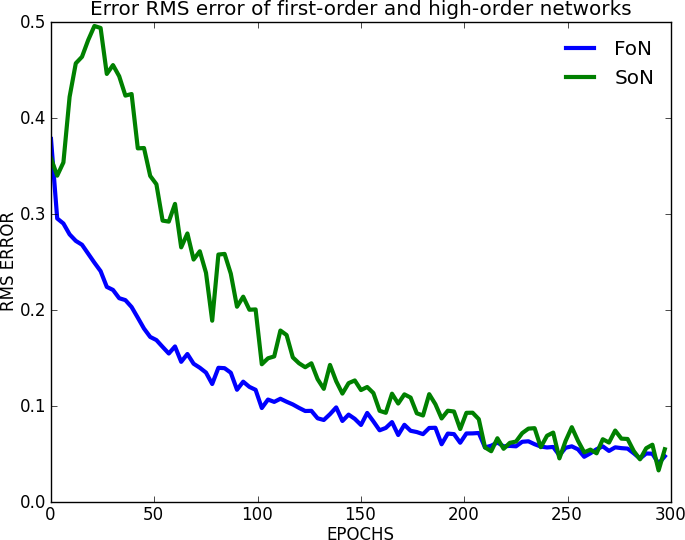
\includegraphics[width=250px]{data/expC2/rms_20.png}
	  &
	  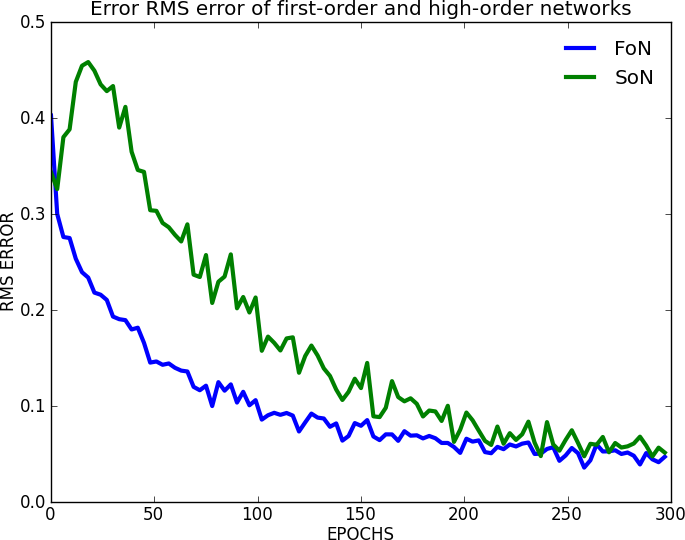
\includegraphics[width=250px]{data/expC2/rms_100.png} \\
	  
	  20 neurones en couche cachée
	  &
	  \hspace*{-1cm}
	  100 neurones en couche cachée
	\end{tabular}
      \end{center} 
      \subparagraph{Notes}
	\begin{itemize}
	  \item formule utilisée pour RMS (cf. Formules~\nameref{rms})
	\end{itemize}
      \subparagraph{Conclusion}
	On remarque que le second réseau apprend et désapprend. De plus, il reste toujours sous la barre
	des 50\%.


  \subsection{Conclusion}
    Le passage sur des données réelles ne modifient pas le comportement du réseau.
    
    
    Cette architecture ouvre des possibilités d'amélioration de l'apprentissage.
    Elle permet au réseau de détecter lui même un nombre de neurones trop important dans la couche cachée.
  
    On pourrait, par exemple, imaginer un réseau s'autorégulant.
  

  \newpage 
  \subsection{Formules}
    \paragraph{RMS} \label{rms}
  Pour une époque $e$ :
  \begin{center}
    \begin{large}
    $ rms_{e} = \sqrt{ \frac{1}{n} \sum \limits_{i=1}^{n} 
    ( o_{i,e} - d_{i} )^2 } $
    \end{large}
  $ with \left\lbrace \begin{array}{lll} n : number\ of\ neurons\ on\ the\ output\ 
  layer\\o_{i,e} : value\ obtained\ for\ the\ i^{th}\ neuron\ at\ the\ e^{th}\ epoch\\d_{i} : 
  value\ desired \ for\ the\ i^{th}\ neuron\end{array} \right.$
  \end{center}
    \paragraph{Descente de gradient} \cite{Touzet_1992} \\
  Construction de l'erreur : 
    \begin{center}
      $y_{i} = f'(a_i) \times ( d_i - x_i ) \ si\ i\ neurone\ de\ sortie $ \\
      $y_{i} = f'(a_i) \times \sum \limits_{k} ( w_{ki} \times y_k )\ si\ i\ neurone\ cache $
    \end{center}
  Mise à jour des poids :
    \begin{center}
      $w_{ij}(t+1) = w_{ij}(t) + learning\_rate \times y_{i} \times x_j + momentum \times 
      (w_{ij}(t) - w_{ij}(t-1) )$
    \end{center}
  Variables : 
    \begin{center}
      $\left\lbrace \begin{array}{lll} 
	f : fonction\ sigmoide \\
	x_i : valeur\ du\ neurone\ i\\
	d_i : valeur\ desire pour\ le\ neurone\ i\\
	a_i : somme\ pondere\ des\ poids\ du\ neurone\ i
      \end{array} \right.$
    \end{center}
    
\bibliographystyle{../pre-rapport/apalike}
\bibliography{../pre-rapport/biblio}
